%!TEX root = ../username.tex
\chapter{Realtime Audio Programming}
\hspace*{-0.15cm}This chapter will consider the theory behind realtime audio programming and the different principles that are followed to create a functional program. It will begin with an overview of digital signal processing. Specifically, this will include the mathematical background required to understand sound. Next, it will cover the methods by which a digital system communicates with several components to create sound. Specifically, this will include how audio data is handled by a digital system's drivers and its corresponding speakers. After, the requirements that a realtime audio program needs in order to function will be considered. This will include a program's typical structure and functionality. Finally, several libraries and other software available that handles these requirements will be discussed in length - focusing primarily on the Virtual Studio Technology Software Development Kit.

\section{Sound As A Discrete Signal}
Sound is a physical phenomenon. Vibrations travel though a medium such as air to create waves and differences in pressure, which travel at the the speed of sound (roughly 331 m/s) \cite{Ling_2016}. These vibrations have varying lengths and intensity depending on the manner in which the sound is created. Changes in frequency are reflected as the pitch of a tone, such as different notes on an instrument. Changes in intensity reflect how loud a particular sound is, such as the different dynamics one can play on an instrument \cite{Ling_2016}. The human brain interprets these differences in pressure by converting waves into electrical signals. When a wave reaches the human ear, the ear canal resonates and converts the sound into mechanical vibrations for the cochlea \cite{Ling_2016}. The cochlea in turn converts these into electrical signals for the brain. Like the human brain, interpreting sound in a digital setting involves simplifying the physical nature of sound waves into a format understandable by computers.

Consider Figure 3.1.

\begin{figure}[h] % [h] used to prevent {figure} from doing weird positioning
\begin{center}
	\fbox{
	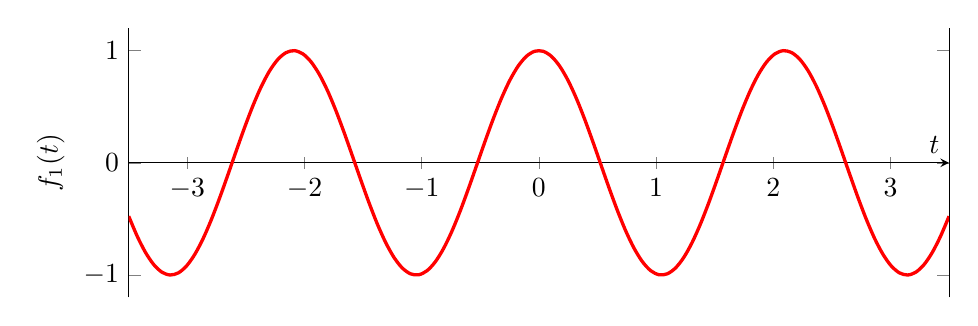
\begin{tikzpicture}
		\begin{axis} [
			axis x line = middle, % The x axis should go through the origin
			xlabel = \(t\),
			ylabel = {\(f_1(t)\)},
			height = 5cm,
			width = 12cm
			]

			\addplot [
			jump mark mid,
			domain = -3.5:3.5,
			samples = 100,
			smooth,
			very thick, red
			] {(cos(deg(3 * x)))};

		\end{axis}
	\end{tikzpicture}}
	\caption{A graph of the wave \(f_1(t) = cos(3t)\).}
\end{center}
\end{figure}

This is a representation of a sinusoid under the time domain. Each crest and trough represent the compressions and rarefactions that occur in real life when this tone is created. By graphing the sinusoid with respect to time, one can view the particular waveform that is created from this given sound. This is an example of a \textit{continuous sinusoidal signal}. They are defined by the following expression:

\begin{defn}[Definition of a continuous sinusoid]\label{def1}
	\begin{equation}\label{introf(t)}
	f(t)=Acos(2\pi ft + \varTheta), t \in (-\infty, \infty)
\end{equation}\end{defn}

where \textit{f} is frequency, \textit{t} is time, and $\varTheta$ is the phase offset in radians \cite{Symons_2013}. By taking the sum of several sinusoids, one can create (or deconstruct) any type of non-sinusoidal signal, given a sufficiently high number of sine waves are used. This is defined as:

\begin{defn}[Definition of a non-sinusoidal continuous signal]\label{def2}
	\begin{equation}\label{intro2f(t)}
	f(t)=\sum_{k=1}^{N_h} A_k cos(2\pi kft + \varTheta_k)
\end{equation}\end{defn}

where \textit{k} is one sinusoid in the sum, $N_h$ is the number of total sinusoids used to construct the signal, $A_k$ the amplitude of a particular signal for each \textit{k}, $\varTheta_k$ the phase for each \textit{k}, and \textit{f} the fundamental frequency of $f(t)$ \cite{Symons_2013}. With this definition in mind, any signal - and therefore, any sound - can be represented as the sum of several sinusoids, seen in Figure 3.2.

\begin{figure}[h] % [h] used to prevent {figure} from doing weird positioning
\begin{center}
	\fbox{
	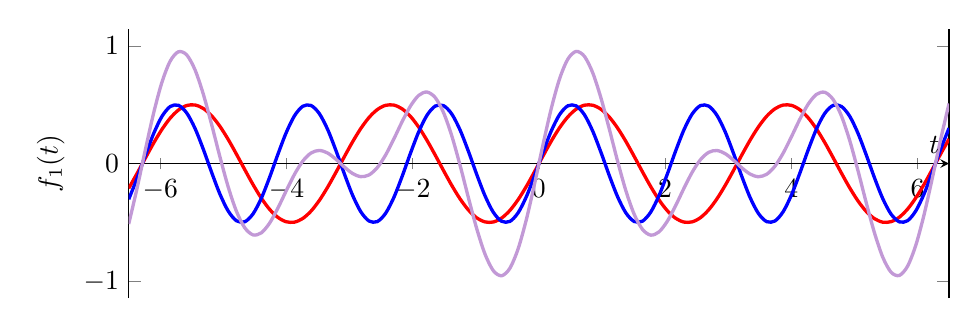
\begin{tikzpicture}
		\begin{axis} [
			axis x line = middle, % The x axis should go through the origin
			xlabel = \(t\),
			ylabel = {\(f_1(t)\)},
			height = 5cm,
			width = 12cm
			]

			\addplot [
			jump mark mid,
			domain=-6.5:6.5,
			samples=100,
			smooth,
			very thick, red
			] {(0.5 * sin(deg(2 * x)))};

			\addplot [
			jump mark mid,
			domain=-6.5:6.5,
			samples=100,
			smooth,
			very thick, blue
			] {(0.5 * sin(deg(3 * x)))};

			\addplot [
			jump mark mid,
			domain=-6.5:6.5,
			samples=100,
			smooth,
			very thick, blue!60!red!40 %xcolor the goat
			] {((0.5 * sin(deg(3 * x))) + (0.5 * (sin(deg(2 * x)))))};
		\end{axis}
	\end{tikzpicture}}
	\caption{A graph of a waveform, deconstructed to its sinusoids.}
\end{center}
\end{figure}

To create a digitial representation of this signal, the \textit{Nyquist-Shannon Sampling Theorem} provides guidelines for how signals should be \textit{bandlimited} - or rather, have their frequencies limited - and how frequently a signal should be sampled to ensure its accuracy.

\begin{defn}[The Nyquist-Shannon Sampling Theorem \cite{Orfanidis_1998}]\label{def3}
\hfill
\begin{enumerate}
	\item The signal must be \textit{bandlimited}, containing no frequencies beyond a particular maximum $F_{max}$.
	\item The \textit{sampling rate} of a signal must be at least twice the maximum frequency $F_{max}$.
\end{enumerate}
\end{defn}

The human ear provides sufficient guidelines for each of these requirements. Typical human hearing spans across a range of 20 Hz - 20,000 Hz \cite{Ling_2016}. As such, the \textit{Nyquist rate} - the minimum sampling rate - for a signal corresponding to an audio waveform must encompass this range. It is defined as $F_s = 2F_{max}$ \cite{Orfanidis_1998}. With an $F_{max} = 20,000$ Hz, the Nyquist rate for audio DSP applications is thus 40,000 Hz. This explains the sample rate for several audio applications. Modern audio recordings use 44,100 Hz, and Digital Audio Workstations usually produce with 48,000 Hz. With this Nyquist rate, the entire range of human hearing is covered.

The process of \textit{sampling} an analog signal is done by taking measurements of a particular function at regular points in time. Each individual measurement of the original analog signal is a \textit{sample}. By convention, samples are in the range (-1,1).

\begin{figure}[h] % [h] used to prevent {figure} from doing weird positioning
	\begin{center}
		\fbox{
		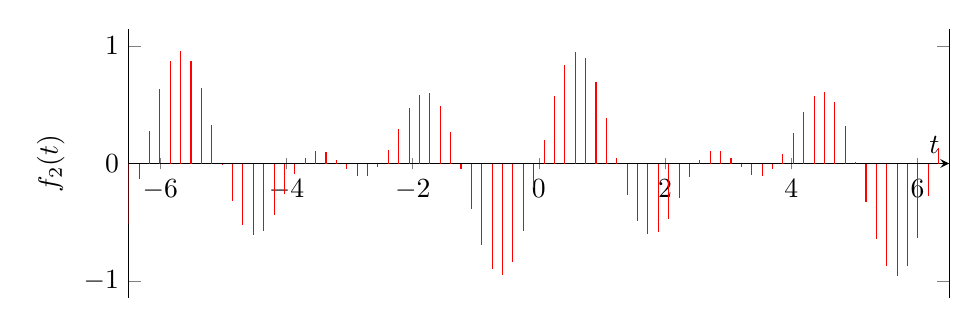
\begin{tikzpicture}
			\begin{axis} [
				axis x line = middle, % The x axis should go through the origin
				xlabel = \(t\),
				ylabel = {\(f_2(t)\)},
				height = 5cm,
				width = 12cm
				]

				\addplot+ [
				ycomb,
				mark = text,
				text mark = , % so jank
				domain = -6.5:6.5,
				samples = 80,
				red
				] {((0.5 * sin(deg(3 * x))) + (0.5 * (sin(deg(2 * x)))))};

			\end{axis}
		\end{tikzpicture}
		}
		\caption{A discrete graph of a waveform taken with 80 samples.}
	\end{center}
\end{figure}

This is a discrete representation of our original continuous signal. Under this representation, one may predict how to represent this in code. If each sample refers to a \textit{float} in the range (-1,1), an array of floats is sufficient to store this waveform in memory. With this representation of sound, one can now use this data to process sound digitally.

\section{The Realtime Programming Bus Schedule}
To process sound digitally, our program has to follow the set schedule requested by the audio driver of the device. It would be impractical to send each sample individually, therefore, a \textit{buffer} of audio data is sent at regular intervals. As buffers of audio data are sent, the integrated sound card of a device accesses the data to be output to the speaker of the device  \cite{Walker_2005}. The smaller the buffer, the less latency there is between audio processing and output. However, this leaves less time to process audio for the digital system. For whatever reason, if data is not available for the sound card to access, the resulting sound will create ``clicks'' and ``pops'' where there is a gap in the audio stream \cite{Walker_2005}. Figure 3.4 describes how this data travels in a digital setting.

\begin{figure}[h] % [h] used to prevent {figure} from doing weird positioning
	\tikzstyle{startstop} = [rectangle, minimum width=3cm, minimum height=1cm,text centered, align=center, draw=black]
	\tikzstyle{arrow} = [thick,->,>=stealth]
	\begin{center}
		\fbox{
		\begin{tikzpicture}
			\node (start) [startstop] {Speakers, Microphones, etc. \\
				\begin{tikzpicture}
					\node (start) [startstop] {DAC};
				\end{tikzpicture}
				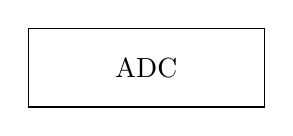
\begin{tikzpicture}
				\node (A) [startstop] {ADC};
				\end{tikzpicture}
			};
			\node (A) [startstop, right of=start, xshift=5cm] {Sound Card \\
			(Generally Integrated)};
			\node (B) [startstop, right of=A, xshift=4cm] {Driver};
			\node (C) [startstop, below of=B, yshift=-1.3cm] {OS \\
			(Win, Mac, etc.)};
			\node (D) [startstop, left of=C, xshift=-4cm] {Audio Driver \\
			(ASIO, Core Audio, etc.)};
			\node (end) [startstop, left of =D, xshift=-5cm] {Host Application \\
				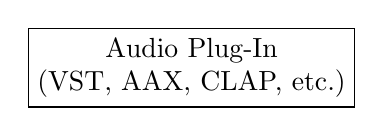
\begin{tikzpicture}
					\node (start) [startstop] {Audio Plug-In \\
					(VST, AAX, CLAP, etc.)};
				\end{tikzpicture}
			};

			\draw [<->, thick] (start) ++(3.2, 0) -- +(0.58, 0);
			\draw [<->, thick] (A) -- node {} (B);
			\draw [<->, thick] (B) -- node {} (C);
			\draw [<->, thick] (C) -- node {} (D);
			\draw [<->, thick] (D) ++(-3.55, 0) -- +(1.14, 0);
		\end{tikzpicture}
		}
		\caption{The flow of information for audio data in a digital system.}
	\end{center}
\end{figure}

Audio is first processed by the audio plugin under a particular host application. This host application is most commonly a \textit{Digital Audio Workstation} (DAW), which handles several different audio plugins to generate and manipulate sound. This audio is then processed by the audio driver into buffers. There are several available drivers that exist, such as ASIO for Windows and Core Audio for Mac (cite). These buffers are sent to the integrated sound card via the OS's drivers, which is sent as output to the system's speakers. Output is completed by the Digital-Audio Converter (DAC) which []. To recieve input, the audio recorded by a microphone connected to the digital system []. The system's [].

This is important to distinguish as a real time program does not simply play audio files akin to one using sound effects for a video game; our program needs to play this sound as it is being generated on-the-fly. This provides limitations that prevent one from using \verb|std::cout| to print information to the terminal during execution, for example. (eh)

\section{Software Available}
There are several libraries and software development kits available that assist in the development of audio plugins, the majority of which use C++. Many of these provide appropriate program structure, classes, and tests that solve the issue of creating a compatible program (mention before?) debugging any issues with one's program. A few popular libraries include:

\begin{enumerate}
	\item JUCE
	\item iPlug2
	\item DISTHRO
\end{enumerate}

These libraries create an abstraction layer that handles several plugin formats. These allow one to create an application [].

These libraries also provide several algorithms that allow one to prototype plugins quickly. []

There are several formats available to programmers [].

The \textit{Virtual Studio Technology} specification allows developers to independently create [], however, the execution of these programs depends on the platform of choice.

\section{The Golden Rules}
The typical structure of a audio program separates the internal processing and the external GUI. This type of structure is more generally known as a \textit{Model View Controller} design pattern. Specifically, the VST SDK uses a variation of this model that combines the view and controller of the model (cite vst sdk doc too) \cite{Bucanek2009}. Figure 3.5 provides a diagram of this. The corresponding interfaces for each part respectively are the \verb|Steinberg::Vst::IAudioProcessor|  and [].

\begin{figure}[h] % [h] used to prevent {figure} from doing weird positioning
	\tikzstyle{startstop} = [rectangle, minimum width=3cm, minimum height=1cm,text centered, align=center, draw=black]
	\tikzstyle{arrow} = [thick,->,>=stealth]
	\begin{center}
		\fbox{
		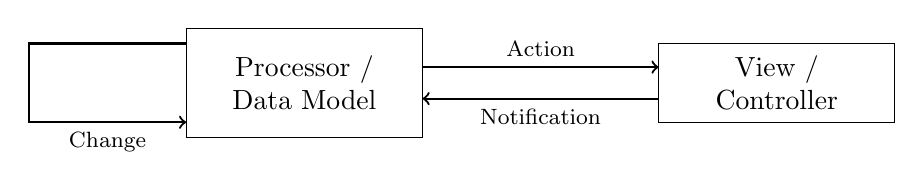
\begin{tikzpicture}
			\node (start) [inner sep=10pt, startstop] {Processor / \\ Data Model};
			\node (A) [startstop, right of=start, xshift=5cm] {View / \\  Controller};

			\draw [->, thick] (start) ++(1.5, 0.2) -- node[anchor=south] {\footnotesize{Action}} +(3, 0) (A);
			\draw [<-, thick] (start) ++(1.5, -0.2) -- node[anchor=north] {\footnotesize{Notification}} +(3, 0) (A);
			\draw [->, thick] (start) ++(-1.5,0.5) -- +(-2,0) -- +(-2,-1) -- node[anchor=north] {\footnotesize{Change}} +(0, -1) (start);
		\end{tikzpicture}
		}
		\caption{The VST SDK Model.}
	\end{center}
\end{figure}

[put more words, eventually talk about UML diagram, maybe in next section?]

\subsection{Development With The VST SDK}
Development in []. Creating a C++ project using the design principles above can be done by using the VST Project Generator. It is a cmake script that [].


\lstset{language =[ANSI]C++}
\lstset{backgroundcolor=\color{white},rulecolor=\color{black}}
\lstset{linewidth=.95\textwidth,breaklines=true}
\lstset{commentstyle=\textit,stringstyle=\upshape,showspaces=false}
\lstset{frame = single}
\lstset{numbers=left,numberstyle=\tiny,basicstyle=\small}
\lstset{commentstyle=\normalfont\itshape,breakautoindent=true}
\lstset{abovecaptionskip=1.2\baselineskip,xleftmargin=30pt}
\lstset{framesep=6pt}
\begin{singlespace}
\lstinputlisting[caption=VST3 Project Generator Script Usage, label=motion]{source/template.txt}
\end{singlespace}

With the design of the plugin taken care of, one can begin implementation of the plugin processor that will manipulate the input signal.
